\documentclass{beamer}

\usepackage{beamerthemeshadow}
\usepackage{amssymb,framed,color,relsize,graphicx,tikz,xcolor}
\usetikzlibrary{angles,quotes}
\usepackage{amsmath}
\usepackage{eucal}
\usepackage{epstopdf}
\usepackage{mathrsfs}
\usepackage[utf8]{inputenc}
\usepackage[T1]{fontenc}
%\usepackage{fontspec}
%\setmainfont{Latin Modern Roman}
%\setsansfont{Latin Modern Sans}
\usepackage{pgfplots}
\usepackage{tikz}
\usepackage{tikz-cd}
\usetikzlibrary{shapes.geometric, decorations.markings, arrows.meta}
\usetikzlibrary{3d,angles,quotes}
\usefonttheme[onlymath]{serif}
\makeatletter

\usetheme{Berlin}
\usecolortheme{UNBC}

\newcommand{\subuni}[0]{\mathrm{Sub}}
\newcommand{\congset}[0]{\mathrm{Con}}
\newcommand{\congen}[2]{\mathrm{Cg}^{#1}({#2})}
\newcommand{\subgen}[2]{\mathrm{Sg}^{#1}({#2})}
\newcommand{\algebra}[1]{\langle {#1} \rangle}
\newcommand{\meet}{\mathrel{\scalebox{0.8}{$\wedge$}}}
\newcommand{\join}{\mathrel{\scalebox{0.8}{$\vee$}}}

\title{The Algebra of Manifolds}
\subtitle{Quillen's Theorem on Cobordism and Formal Groups}
\titlegraphic{
\includegraphics[width=5cm]{logo_green.jpeg}}
\author{Deepak Jassal}
\institute[UNBC]{University of Northern British Columbia\\MATH 420 Structure of Groups and Rings}
\date{April 5\textsuperscript{th}, 2026}

\begin{document}

\begin{frame}
  \titlepage
\end{frame}

\section{Background}

\begin{frame}{What is a Manifold?}
  \begin{block}{Idea}
    A \textbf{manifold} is a space that looks locally like Euclidean space $\mathbb{R}^n$.
  \end{block}
  \begin{columns}[T]
    \column{0.5\textwidth}
      \textbf{Examples:}
      \begin{itemize}
        \item A circle ($S^1$) – locally looks like $\mathbb{R}$
        \item A sphere ($S^2$) – locally looks like $\mathbb{R}^2$
        \item The surface of a donut (torus)
        \item A saddle
      \end{itemize}
    \column{0.5\textwidth}
      \begin{center}
      \begin{tikzpicture}[scale=0.8]
          \draw (0,0) circle (1);
          \node at (0,-1.5) {Circle $S^1$};
      \end{tikzpicture}
      \begin{tikzpicture}[scale=0.5]
          \draw (0,0) circle (1);
          \draw (0,0) ellipse (1 and 0.4);
          \node at (0,-1.8) {Sphere $S^2$};
      \end{tikzpicture}
      \end{center}
  \end{columns}
  \vfill
  \begin{quote}
  \centering
  ``A manifold is a space where every point has a neighborhood that looks like $\mathbb{R}^n$.''
  \end{quote}
\end{frame}

\begin{frame}{Complex Manifolds}
  \begin{block}{Idea}
    A \textbf{complex manifold} is a manifold that locally looks like $\mathbb{C}^n$ instead of $\mathbb{R}^n$.
  \end{block}
  \begin{columns}[T]
    \column{0.3\textwidth}
      This can be thought of as the space locally being $\mathbb{R}^{2n}$.\\
      The gridlines show that the torus locally looks like $\mathbb{C}$ or $\mathbb{R}^{2}$.
    \column{0.7\textwidth}
      \begin{tikzpicture}[scale=1]
          \begin{axis}[hide axis, axis lines=none, axis equal=true,]
            \addplot3[surf,
            colormap/cool,
            samples=20,
            domain=0:2*pi,y domain=0:2*pi,
            z buffer=sort]
            ({(2+cos(deg(x)))*cos(deg(y+pi/2))}, 4
              {(2+cos(deg(x)))*sin(deg(y+pi/2))}, 
              {sin(deg(x))});
          \end{axis}
      \end{tikzpicture}
  \end{columns}  
\end{frame}

\begin{frame}{What is a Vector Bundle?}
  \begin{block}{Idea}
    A \textbf{vector bundle} is a family of vector spaces continuously attached to each point of a manifold.
  \end{block}
  \begin{center}
  \begin{tikzpicture}[scale=0.8]
      \draw[thick] (0,0) to [bend left] (4,0);
      \draw[thick] (0,0) to [bend right] (4,0);
      \node at (2,-0.8) {Base manifold $X$};
      \draw[<->] (1,0.5) -- (1,1.5);
      \draw[<->] (2,0.3) -- (2,1.8);
      \draw[<->] (3,0.5) -- (3,1.5);
      \node at (3.5,1.8) {Fiber $\mathbb{R}^n$};
  \end{tikzpicture}
  \end{center}
  \vfill
  \textbf{Example:} The \textbf{tangent bundle} of a sphere - at each point, attach the tangent plane.
  \begin{itemize}
    \item A \textbf{line bundle} is when each fiber is 1-dimensional (a line).
  \end{itemize}
\end{frame}

\begin{frame}{Vector Bundles}
  \begin{definition}
    A \textbf{vector bundle} of rank $n$ over $\mathbb{F} \in \{\mathbb{R}, \mathbb{C}\}$ is a triple $(E, X, \pi)$ where:
    \begin{itemize}
        \item $E$ (total space) and $X$ (base) are spaces/manifolds
        \item $\pi: E \to X$ is a continuous/smooth map
        \item For each $x \in X$, $\pi^{-1}(x) \cong \mathbb{F}^n$ (a vector space)
        \item \textbf{Local triviality:} $\forall x \in X$, $\exists$ neighborhood $U$ with $\pi^{-1}(U) \cong U \times \mathbb{F}^n$
    \end{itemize}
  \end{definition}
\end{frame}

\begin{frame}{The M\"obius Strip}
  \begin{columns}
    \column{0.5\textwidth}
      Locally vector bundles look like $U\times V$.\\
      But globally they can be twisted.
    \column{0.5\textwidth}
      \begin{figure}
        \centering
        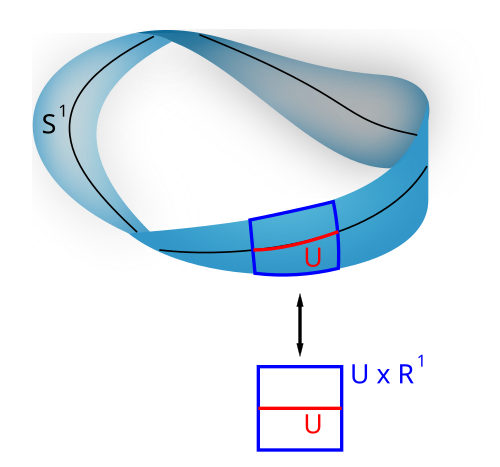
\includegraphics[width=1\textwidth]{MobiusStrip.png}
        \caption{Wikipedia}
      \end{figure}
  \end{columns}
\end{frame}

\begin{frame}{Cycles}
  \begin{block}{The Intuition}
  A \textbf{$n$-cycle} is an $n$-dimensional shape with \textbf{no boundary}.
  \begin{itemize}
    \item 1-cycle: A loop (circle) — no endpoints
    \item 2-cycle: A sphere — no edges
  \end{itemize}
  \emph{Slogan: "A soap bubble with no holes in the film itself."}
  \end{block}
  \begin{block}{Cycles Detect Holes}
  \begin{itemize}
    \item A cycle that can be shrunk to a point is a \textbf{boundary} (it bounds something higher-dimensional)
    \item A cycle that cannot be shrunk \textbf{detects a hole}
  \end{itemize}
  \end{block}
\end{frame}

\begin{frame}{Examples of Cycles}
  \begin{columns}
    \column{0.5\textwidth}
      \begin{itemize}
        \item Circle on a sphere: Can shrink → trivial (no hole)
        \item Circle around a torus: Cannot shrink → detects a hole
      \end{itemize}
    \column{0.5\textwidth}
      Cyles that are not boundaries are holes
  \end{columns}
\end{frame}

\begin{frame}{Homology}
  \begin{block}{Homology ($H_n(X)$)}
    Measures the \textbf{$n$-dimensional holes} in a space $X$.\\
    Essentially the number of $n$-dimensional cycles modulo $n$-dimensional boundaries.
    \begin{itemize}
      \item $H_0$: Number of connected components
      \item $H_1$: Loops that cannot be pulled tight (tunnels)
    \end{itemize}
    \[
      H_n(X) = \frac{\{\text{$n$-dimensional cycles}\}}{\{\text{$n$-dimensional boundaries}\}}
    \]
  \end{block}
\end{frame}

\begin{frame}{Cohomology}
  \begin{block}{Cohomology ($H^n(X)$)}
    The \textbf{dual} of homology — assigns numbers to holes in a consistent way.
    \begin{itemize}
      \item Has a \textbf{product} (cup product) — forms a \textbf{ring}
      \item Essential for characteristic classes and formal group laws
    \end{itemize}
  \end{block}
\end{frame}

\section{Cobordism}

\begin{frame}{Formal Group Law}
  \begin{definition}
    A \textbf{(commutative) formal group law} over a ring $R$ is a power series $F(T_1,T_2)\in R[[T_1,T_2]]$ satisfying
    \begin{enumerate}
      \item \textbf{Identity:} $F(T,0)=F(0,T)=T$
      \item \textbf{Associativity:} $F(T_1,F(T_2,T_3))=F(F(T_1,T_2),T_3)$
      \item \textbf{Commutativity:} $F(T_1,T_2)=F(T_2,F_1)$ 
    \end{enumerate}
  \end{definition}    
\end{frame}

\begin{frame}{Bordism and Cobordism}
  \begin{definition}
    Two closed manifolds $M$ and $N$ are \textbf{cobordant} if their disjoint union forms the entire boundary of some higher-dimensional manifold $W$.
    \[
      \partial W = M \sqcup N
    \]
  \end{definition}
  \textbf{Examples:}
  \begin{itemize}
    \item A circle bounds a disk.
    \item Two circles bound a ``pair of pants'' (cylinder).
    \item Any closed manifold bounds something? No!
  \end{itemize}
\end{frame}

\begin{frame}{The Cobordism Ring}
  \begin{block}{Construction (Complex Cobordism $MU_*$ or $U^*(pt)$)}
  Take all closed smooth manifolds with a \textbf{stable complex structure}.
  \begin{itemize}
    \item \textbf{Addition:} Disjoint union $\sqcup$
    \item \textbf{Multiplication:} Cartesian product $\times$
    \item \textbf{Zero:} Empty manifold
  \end{itemize}
  \end{block}
  \vfill
  \begin{alertblock}{The Big Question (1960s)}
  What is the algebraic structure of this ring?
  \[
    MU_*=\bigoplus_{n\geq0} MU_n
  \]
  \end{alertblock}
\end{frame}

\begin{frame}{What is an Euler Class?}
  \begin{block}{Euler Classes}
  The \textbf{Euler class} $e(E)$ measures the obstruction to finding a nowhere-zero section of a vector bundle $E$.
  \begin{itemize}
    \item $e(E) = 0$ $\Rightarrow$ you can "comb the hair" (nowhere-zero section exists)
    \item $e(E) \neq 0$ $\Rightarrow$ you cannot (every section has a zero)
  \end{itemize}
  \end{block}
\end{frame}

\begin{frame}{The Formal Group Law of Cobordism}
  \begin{block}{Euler Classes}
    For complex line bundles $L_1, L_2$, the Euler class satisfies:
    \[
      e(L_1 \otimes L_2) = F(e(L_1), e(L_2))
    \]
    where $F$ is a \textbf{formal group law} with coefficients $a_{ij} \in U^*(pt)$.
  \end{block}
  \begin{block}{Key Observation}
    The cobordism ring $U^*(pt)$ \textbf{has} a formal group law $F_U$ coming from tensor product of line bundles.
  \end{block}
  \begin{quote}
    \small So $U^*(pt)$ is not just a ring — it comes equipped with a formal group law.
  \end{quote}
\end{frame}

\section{Main Results}

\begin{frame}{Lazard's Theorem}
  \begin{theorem}
   \begin{enumerate}
    \item There exists a \textbf{universal} formal group law $F_{univ}$ over a ring $L$
    \item Any formal group law over any ring $R$ comes from a unique map $L \to R$
    \item $L$ is a polynomial ring: $L \cong \mathbb{Z}[t_1, t_2, t_3, \dots]$ with $\deg t_i = 2i$
  \end{enumerate}   
  \end{theorem}

  \begin{quote}
    \small Lazard's theorem is \textbf{pure algebra} — no topology involved.
  \end{quote}
\end{frame}

\begin{frame}{Applying Lazard's Theorem}
  \begin{block}{By Lazard's Universality}
    Since $U^*(pt)$ has a formal group law $F_U$, there exists a \textbf{unique} ring homomorphism:
    \[
      \phi: L \longrightarrow U^*(pt)
    \]
    sending the universal formal group law $F_{univ}$ to $F_U$.
  \end{block}
  \begin{center}
    \begin{tikzpicture}
      \node (L) at (0,0) {$L$};
      \node (U) at (4,0) {$U^*(pt)$};
      \node (Funiv) at (0,-1) {$F_{univ}$};
      \node (FU) at (4,-1) {$F_U$};
      \draw[->] (L) -- (U) node[midway, above] {$\phi$};
      \draw[->] (Funiv) -- (FU) node[midway, above] {$\phi_*$};
    \end{tikzpicture}
  \end{center}
  \begin{block}{What is $\phi$?}
    $\phi$ sends each universal coefficient $t_i \in L$ to some cobordism class in $U^*(pt)$.
  \end{block}
  \begin{quote}
    \small Lazard gives us a \textbf{map} from the universal ring to the cobordism ring.
  \end{quote}
\end{frame}

\begin{frame}{Quillen's Theorem (1971)}
  \begin{alertblock}{Quillen's Theorem}
    The homomorphism $\phi: L \to U^*(pt)$ is an \textbf{isomorphism}.
  \end{alertblock}
  \begin{block}{Consequences}
    \[
      U^*(pt) \cong L \cong \mathbb{Z}[x_2, x_4, x_6, x_8, \dots]
    \]
    where deg $x_{2n}$ is $-2n$ (or $MU_{2n}$ in homology grading).
  \end{block}
  \begin{block}{What This Means}
  \begin{itemize}
    \item The cobordism ring is a \textbf{polynomial ring}
    \item One generator in each even dimension: $x_2 = [\mathbb{CP}^1]$, $x_4 = [\mathbb{CP}^2]$, etc.
    \item The formal group law of cobordism is the \textbf{universal} one
  \end{itemize}
  \end{block}
\end{frame}

\begin{frame}{What Does This Mean Geometrically?}
  \begin{block}{Concrete Interpretation}
    There exist manifolds $M_2, M_4, M_6, \dots$ (one in each even dimension) such that \textbf{every} complex manifold is cobordant to a unique polynomial combination of products of these generators.
  \end{block}
  \vfill
  \textbf{Analogy:}
  \begin{itemize}
    \item Integers $\mathbb{Z}$ are generated by prime numbers.
    \item Cobordism ring is generated by these special manifolds.
  \end{itemize}
  \vfill
  \textbf{Example generators:}
  \begin{itemize}
    \item $x_2$: $\mathbb{CP}^1$ (the Riemann sphere)
    \item $x_4$: $\mathbb{CP}^2$ (complex projective plane)
  \end{itemize}
\end{frame}

\begin{frame}{Summary}
  \begin{theorem}[Quillen, 1971]
  The complex cobordism ring $U^*(pt)$ is isomorphic to Lazard's universal ring $L$:
  \[
    U^*(pt) \cong \mathbb{Z}[x_2, x_4, x_6, \dots]
  \]
  \end{theorem}
  \begin{center}
    \textbf{Key Idea:} The formal group law arising from tensor products of line bundles over manifolds is the \textit{most general possible}.
  \end{center}
  \vfill
  \begin{flushright}
    \textsc{Thank you!}
  \end{flushright}
\end{frame}

\end{document}